%==============================================================================
% Praca dyplomowa (UR) — plik główny
%==============================================================================

\documentclass{urdpl}

%------------------------------------------------------------------------------
% JĘZYK / KODOWANIE (pdfLaTeX)
%------------------------------------------------------------------------------
\usepackage[main=polish,english]{babel}
\usepackage[utf8]{inputenc} % tylko pdfLaTeX

%------------------------------------------------------------------------------
% MATEMATYKA
%------------------------------------------------------------------------------
\usepackage{mathtools}


%------------------------------------------------------------------------------
% HYPERLINKI
%------------------------------------------------------------------------------
\usepackage[hidelinks]{hyperref}

%------------------------------------------------------------------------------
% FLOATY (tylko jeśli używasz [H])
%------------------------------------------------------------------------------
\usepackage{float}

%------------------------------------------------------------------------------
% TABELE (wg potrzeby)
%------------------------------------------------------------------------------
\usepackage{multirow}
\usepackage{array}
\usepackage{makecell}
\usepackage[flushleft]{threeparttable}
\usepackage{colortbl}
\definecolor{tableheader}{RGB}{198, 217, 241}

%------------------------------------------------------------------------------
% PODKREŚLANIE + NUMERY LINII (opcjonalnie)
%------------------------------------------------------------------------------
\usepackage[normalem]{ulem}
\usepackage{lineno}

%------------------------------------------------------------------------------
% CYTOWANIA
%------------------------------------------------------------------------------
\usepackage{csquotes}

%------------------------------------------------------------------------------
% METADANE PRACY (dla urdpl.cls)
%------------------------------------------------------------------------------
\author{Dominik Kuraś}
\shortauthor{D. Kuraś}
\noAlbum{134939}

\titlePL{Mobilny dziennik tankowań i eksploatacji pojazdów\\\textit{MotoLog}}
\titleEN{Mobile log of refueling and vehicle operation\\\textit{MotoLog}} % Podajemy tytuł w obu językach

\shorttitlePL{MotoLog -- mobilny dziennik pojazdu}
\shorttitleEN{MotoLog -- Mobile Vehicle Log}

\thesistype{Praca projektowa}
\thesisDone{Prowadzący zajęcia laboratoryjne: }
\supervisor{dr inż. Przemysław Pardel}

\degreeprogramme{Informatyka}

\date{2027}

\department{Instytut Informatyki}
\faculty{Wydział Nauk Ścisłych i Technicznych}

%druga strona mozna cos dopisac
% \acknowledgements{Serdecznie dziękuję \dots } % dowolnośc mozńa usunąć

%------------------------------------------------------------------------------
% USTAWIENIA NUMERACJI I SPISU TREŚCI
%------------------------------------------------------------------------------
\setcounter{secnumdepth}{1} % numeruje tylko do \section (np. 2.1), wyłącza numerki przy \subsection (2.1.1) i niżej
\setcounter{tocdepth}{1}    % w spisie treści pokazuje tylko do \section, ukrywa \subsection i niżej


%==============================================================================
\begin{document}
%==============================================================================


%------------------------------------------------------------------------------
% Strona tytułowa + podziękowania
%------------------------------------------------------------------------------
\titlepages


%------------------------------------------------------------------------------
% Streszczenie (PL) – NIE dodajemy do spisu treści
%------------------------------------------------------------------------------
 
\cleardoublepage
\selectlanguage{polish}
\chapter*{Streszczenie pracy}
\label{cha:streszczenie-pl}

Streszczenie pracy w języku polskim.

%------------------------------------------------------------------------------
% Abstract (EN) – NIE dodajemy do spisu treści
%------------------------------------------------------------------------------
 
\cleardoublepage
\selectlanguage{english}
\chapter*{Abstract}
\label{cha:abstract-en}


Abstract thesis ...


%------------------------------------------------------------------------------
% Spis treści
%------------------------------------------------------------------------------
\selectlanguage{polish}
\tableofcontents

\clearpage
\linenumbers % jeśli nie chcesz numerów linii w całości, usuń lub przenieś

%------------------------------------------------------------------------------
% Rozdziały
%------------------------------------------------------------------------------
\chapter{Analiza problemu i przegląd istniejących rozwiązań}
\label{cha:analiza_problemu}

Utrzymanie samochodu to nie tylko regularne tankowanie czy ładowanie, ale też serwis, ubezpieczenia, przeglądy i~raty leasingowe. Wielu kierowców zapisuje te koszty na papierowych paragonach, w~luźnych notatkach albo próbuje je po prostu zapamiętać. Takie rozproszenie utrudnia policzenie realnych wydatków na auto i~wyłapanie nagłego wzrostu spalania, który często sygnalizuje usterkę. Problem rośnie, gdy w~domu jest kilka pojazdów, a~o~kończącej się polisie OC czy badaniu technicznym łatwo zapomnieć.

% ==============================================================================
\section{Uzasadnienie potrzeby opracowania rozwiązania}
\label{sec:uzasadnienie_rozwiazania}

Dostępne na rynku aplikacje do kontroli wydatków na auto nie zawsze sprawdzają się w~codziennym użyciu. Wiele z~nich wymaga założenia konta i~stałego dostępu do Internetu, co utrudnia szybki zapis danych na stacji paliw ze słabym zasięgiem albo w~garażu podziemnym. Część darmowych narzędzi blokuje obsługę kilku pojazdów i~skanowanie paragonów za płatną subskrypcją lub zasypuje ekran reklamami.

Projektowana aplikacja \textbf{MotoLog} rozwiązuje te problemy, przenosząc zapis i~przetwarzanie danych bezpośrednio na telefon użytkownika. Dzięki temu system działa szybko, bez konieczności rejestracji i~niezależnie od połączenia z~siecią.

\subsection{Główne cele projektowanego systemu}
\label{subsec:glowne_cele}

Głównym celem jest uproszczenie zapisu tankowań i~ładowań dzięki odczytowi paragonów (OCR) oraz automatycznemu wyliczaniu średniego zużycia paliwa lub energii i~zasięgu auta. Aplikacja ma też porządkować wydatki poprzez podział na kategorie, historię wpisów oraz prognozę miesięcznego budżetu. Ważnym założeniem jest obsługa kilku pojazdów o~różnych napędach oraz wysyłanie lokalnych powiadomień, które chronią przed przegapieniem terminów opłat i~przeglądów.

Szczegółową analizę problemów biznesowych, zakres projektu oraz pełną listę wymagań i~reguł działania systemu opisano w~Rozdziale~\ref{cha:analiza_wymagan}.


% % ==============================================================================
% \section{Przegląd istniejących rozwiązań}
% \label{sec:przeglad_rozwiazan}

% \subsection{Analiza wybranych aplikacji}
% \label{subsec:analiza_aplikacji}

% \subsubsection{Rozwiązanie 1 (np. https://spalanie.formuly.pl/)}
% \label{subsubsec:rozwiazanie_1}
% % TODO: Opis, funkcjonalności, zalety oraz ograniczenia pierwszego rozwiązania.

% \subsubsection{Rozwiązanie 2 (np. Drivvo)}
% \label{subsubsec:rozwiazanie_2}
% % TODO: Opis, funkcjonalności, zalety oraz ograniczenia drugiego rozwiązania.

% \subsubsection{Rozwiązanie 3 (np. Yanosik)}
% \label{subsubsec:rozwiazanie_3}
% % TODO: Opis, funkcjonalności, zalety oraz ograniczenia trzeciego rozwiązania.


% \subsection{Porównanie analizowanych systemów}
% \label{subsec:porownanie_rozwiazan}

% Zestawienie porównawcze przeanalizowanych rozwiązań przedstawiono w~tabeli~\ref{tab:porownanie_rozwiazan}.

% \begingroup
% \renewcommand{\arraystretch}{1.3}
% \setlength{\LTcapwidth}{\linewidth}
% \begin{longtable}{|>{\centering\arraybackslash}m{2.8cm}|*{3}{m{\dimexpr(\linewidth - 2.8cm - 10\tabcolsep - 6\arrayrulewidth)/4\relax}|}>{\bfseries}m{\dimexpr(\linewidth - 2.8cm - 10\tabcolsep - 6\arrayrulewidth)/4\relax}|}
%     \caption{Porównanie istniejących rozwiązań z~projektowanym systemem}
%     \label{tab:porownanie_rozwiazan} \\
%     \hline
%     \rowcolor{tableheader}
%     \textbf{Cecha / Kryterium} & \multicolumn{1}{c|}{\textbf{Rozwiązanie A}} & \multicolumn{1}{c|}{\textbf{Rozwiązanie B}} & \multicolumn{1}{c|}{\textbf{Rozwiązanie C}} & \multicolumn{1}{c|}{\textbf{MotoLog (Projekt)}} \\
%     \hline
%     \endfirsthead

%     \multicolumn{5}{c}{\footnotesize\bfseries \tablename\ \thetable{} -- kontynuacja z~poprzedniej strony} \\
%     \hline
%     \rowcolor{tableheader}
%     \textbf{Cecha / Kryterium} & \multicolumn{1}{c|}{\textbf{Rozwiązanie A}} & \multicolumn{1}{c|}{\textbf{Rozwiązanie B}} & \multicolumn{1}{c|}{\textbf{Rozwiązanie C}} & \multicolumn{1}{c|}{\textbf{MotoLog (Projekt)}} \\
%     \hline
%     \endhead

%     \multicolumn{5}{r}{\footnotesize\emph{Ciąg dalszy na następnej stronie\ldots}} \\
%     \endfoot

%     \zrodloLT{5}{Opracowanie własne.}
%     \endlastfoot

%     \textbf{Główne funkcjonalności} & 
%     & 
%     & 
%     & \\
%     \hline
%     \textbf{Zalety} & 
%     & 
%     & 
%     & \\
%     \hline
%     \textbf{Ograniczenia} & 
%     & 
%     & 
%     & \\
%     \hline
%     \textbf{Działanie offline} & 
%     & 
%     & 
%     & \\
%     \hline
% \end{longtable}
% \endgroup

% % ==============================================================================
% \section{Wyróżniki projektowanego systemu}
% \label{sec:wyrozniki_systemu}

% % TODO: Elementy wyróżniające projektowany system na tle istniejących rozwiązań
% \begin{itemize}
%     \item \textbf{Element 1} -- % opis...
%     \item \textbf{Element 2} -- % opis...
%     \item \textbf{Element 3} -- % opis...
% \end{itemize}





% ==============================================================================
\section{Przegląd istniejących rozwiązań}
\label{sec:przeglad_rozwiazan}

W~niniejszym podrozdziale przeanalizowano pięć istniejących narzędzi wspierających kierowców w~kontroli zużycia paliwa oraz kosztów utrzymania pojazdu: kalkulator przeglądarkowy \textbf{spalanie.formuly.pl}, aplikacje mobilne \textbf{Drivvo} i~\textbf{Yanosik} oraz platformy webowo-mobilne \textbf{Fuelly} i~\textbf{Spritmonitor}.

\subsection{Analiza wybranych aplikacji}
\label{subsec:analiza_aplikacji}

% ------------------------------------------------------------------------------
\subsubsection{Rozwiązanie 1: spalanie.formuly.pl}
\label{subsubsec:rozwiazanie_1}

\textbf{Charakterystyka i~dostępność.} Serwis \textbf{spalanie.formuly.pl} to prosty kalkulator internetowy dostępny wyłącznie przez przeglądarkę WWW na komputerach i~urządzeniach mobilnych. Narzędzie nie posiada dedykowanych aplikacji natywnych w~sklepach Google Play i~App Store ani modułu rejestracji konta. Korzystanie ze strony jest bezpłatne, a~w~interfejsie mogą pojawiać się standardowe banery reklamowe.

\textbf{Zakres funkcji i~obsługa procesu.} Aplikacja działa w~modelu bezstanowym i~nie przechowuje historii wpisów ani profili pojazdów. Użytkownik wpisuje w~pojedynczym formularzu ilość zatankowanego paliwa, przejechany dystans oraz cenę za litr, a~system oblicza średnie spalanie na 100~km oraz koszt przejazdu. Serwis nie obsługuje wielu pojazdów, ewidencji wydatków serwisowych i~ubezpieczeniowych, wykresów trendów, przypomnień o~terminach, eksportu danych ani integracji z~innymi usługami.

\textbf{Ocena użyteczności i~prywatności.} Interfejs ogranicza się do jednego formularza, dzięki czemu obsługa jest natychmiastowa i~nie wymaga podawania żadnych danych osobowych. Brak lokalnej bazy wymusza jednak stały dostęp do Internetu przy każdym użyciu. Rozwiązanie sprawdza się wyłącznie jako doraźny kalkulator dla jednego przejazdu i~nie nadaje się do długoterminowej kontroli budżetu ani prowadzenia kilku aut.

\begin{figure}[H]
    \centering
    % \includegraphics[width=0.85\linewidth]{figures/spalanie_formuly_glowny.png}
    \caption{Widok główny kalkulatora w~serwisie spalanie.formuly.pl}
    \label{fig:spalanie_formuly_glowny}
    \zrodlo{Opracowanie własne na podstawie widoku aplikacji WWW (brak oddzielnych ekranów pojazdów, raportów, wydatków i~przypomnień ze względu na bezstanowy charakter narzędzia).}
\end{figure}

% ------------------------------------------------------------------------------
\subsubsection{Rozwiązanie 2: Drivvo}
\label{subsubsec:rozwiazanie_2}

\textbf{Charakterystyka i~dostępność.} \textbf{Drivvo} to rozbudowany dziennik eksploatacji pojazdu dostępny jako aplikacja mobilna na systemy Android i~iOS oraz poprzez panel przeglądarkowy WWW. Korzystanie z~systemu w~podstawowym zakresie jest darmowe po utworzeniu konta użytkownika (za pomocą adresu e-mail lub logowania społecznościowego), przy czym w~wersji bezpłatnej wyświetlane są reklamy. Producent udostępnia również płatny wariant rozszerzony, który usuwa reklamy oraz odblokowuje zaawansowane raportowanie, kopie zapasowe i~eksport danych.

\textbf{Zakres funkcji i~obsługa procesu.} Dodanie pojazdu wymaga określenia jego typu, marki, modelu, rodzaju paliwa oraz początkowego stanu licznika. System obsługuje wiele pojazdów w~ramach jednego profilu i~pozwala rejestrować tankowania z~automatycznym wyliczeniem średniego zużycia paliwa. Ewidencja kosztów obejmuje szeroką listę kategorii, w~tym naprawy serwisowe, wymianę oleju i~opon, ubezpieczenia, podatki, myjnię, parkingi oraz opłaty drogowe. Aplikacja generuje wykresy wydatków i~spalania w~czasie, wysyła przypomnienia powiązane z~datą lub przebiegiem oraz umożliwia eksport zestawień do plików CSV i~arkuszy kalkulacyjnych.

\textbf{Ocena użyteczności i~prywatności.} Bogaty zestaw funkcji analitycznych sprawia, że interfejs wymaga chwili na opanowanie struktury menu i~kategorii. Dane użytkowników są synchronizowane z~chmurą producenta, co ułatwia przeniesienie historii na nowe urządzenie, ale wiąże się z~przechowywaniem informacji poza telefonem. Dla zwykłego kierowcy wersja darmowa bywa uciążliwa z~powodu reklam, natomiast dla osób zarządzających kilkoma autami aplikacja oferuje bardzo szerokie możliwości ewidencyjne.

\begin{figure}[H]
    \centering
    % \includegraphics[width=0.45\linewidth]{figures/drivvo_glowny.png}
    % \includegraphics[width=0.45\linewidth]{figures/drivvo_pojazd.png}
    \caption{Aplikacja Drivvo: ekran główny oraz formularz dodawania pojazdu}
    \label{fig:drivvo_1}
    \zrodlo{Zrzuty ekranu z~aplikacji Drivvo.}
\end{figure}

\begin{figure}[H]
    \centering
    % \includegraphics[width=0.45\linewidth]{figures/drivvo_tankowanie.png}
    % \includegraphics[width=0.45\linewidth]{figures/drivvo_raporty.png}
    \caption{Aplikacja Drivvo: rejestracja tankowania oraz widok raportów i~statystyk}
    \label{fig:drivvo_2}
    \zrodlo{Zrzuty ekranu z~aplikacji Drivvo.}
\end{figure}

\begin{figure}[H]
    \centering
    % \includegraphics[width=0.45\linewidth]{figures/drivvo_wydatki.png}
    % \includegraphics[width=0.45\linewidth]{figures/drivvo_przypomnienia.png}
    \caption{Aplikacja Drivvo: ewidencja wydatków oraz konfiguracja przypomnień}
    \label{fig:drivvo_3}
    \zrodlo{Zrzuty ekranu z~aplikacji Drivvo.}
\end{figure}

% ------------------------------------------------------------------------------
\subsubsection{Rozwiązanie 3: Yanosik}
\label{subsubsec:rozwiazanie_3}

\textbf{Charakterystyka i~dostępność.} \textbf{Yanosik} to polska aplikacja mobilna na platformy Android oraz iOS, łącząca nawigację drogową i~system ostrzegania kierowców z~modułem obsługi pojazdu. Podstawowe funkcje drogowe są darmowe, jednak interfejs zawiera liczne banery reklamowe oraz oferty usług partnerskich. Dostępne są płatne pakiety rozszerzające funkcje asystenta jazdy i~ograniczające reklamy.

\textbf{Zakres funkcji i~obsługa procesu.} Korzystanie z~nawigacji nie wymaga logowania, natomiast zapisanie profilu pojazdu i~obsługa przypomnień wymagają założenia konta. W~sekcji pojazdu kierowca wprowadza numer rejestracyjny, markę, model oraz daty ważności polisy OC i~badania technicznego, z~możliwością dodania kilku samochodów. Aplikacja powiadamia o~zbliżających się terminach ubezpieczenia i~przeglądu oraz pozwala zapisywać podstawowe wydatki, jednak nie oferuje wyspecjalizowanej analityki spalania między pełnymi tankowaniami, skanowania paragonów OCR ani eksportu szczegółowych raportów kosztowych. System integruje się z~urządzeniami pokładowymi producenta oraz interfejsami Android Auto i~Apple CarPlay.

\textbf{Ocena użyteczności i~prywatności.} Ekran główny jest podporządkowany obsłudze w~trakcie jazdy, przez co funkcje typowo księgowe znajdują się głębiej w~menu. Aplikacja wymaga stałego połączenia z~siecią i~dostępu do lokalizacji, przetwarzając dane telemetryczne na serwerach operatora. Z~punktu widzenia zwykłego kierowcy jest to wygodny asystent uniwersalny, ale jako narzędzie do precyzyjnego rozliczania spalania i~kosztów wielu pojazdów wypada słabiej od dedykowanych dzienników.

\begin{figure}[H]
    \centering
    % \includegraphics[width=0.45\linewidth]{figures/yanosik_glowny.png}
    % \includegraphics[width=0.45\linewidth]{figures/yanosik_pojazd.png}
    \caption{Aplikacja Yanosik: ekran główny oraz moduł dodawania pojazdu}
    \label{fig:yanosik_1}
    \zrodlo{Zrzuty ekranu z~aplikacji Yanosik.}
\end{figure}

\begin{figure}[H]
    \centering
    % \includegraphics[width=0.45\linewidth]{figures/yanosik_tankowanie.png}
    % \includegraphics[width=0.45\linewidth]{figures/yanosik_raporty.png}
    \caption{Aplikacja Yanosik: rejestracja kosztów paliwa oraz podsumowanie wydatków}
    \label{fig:yanosik_2}
    \zrodlo{Zrzuty ekranu z~aplikacji Yanosik.}
\end{figure}

\begin{figure}[H]
    \centering
    % \includegraphics[width=0.45\linewidth]{figures/yanosik_wydatki.png}
    % \includegraphics[width=0.45\linewidth]{figures/yanosik_przypomnienia.png}
    \caption{Aplikacja Yanosik: lista wydatków oraz przypomnienia o~terminach OC i~przeglądu}
    \label{fig:yanosik_3}
    \zrodlo{Zrzuty ekranu z~aplikacji Yanosik.}
\end{figure}

% ------------------------------------------------------------------------------
\subsubsection{Rozwiązanie 4: Fuelly}
\label{subsubsec:rozwiazanie_4}

\textbf{Charakterystyka i~dostępność.} \textbf{Fuelly} to platforma do śledzenia zużycia paliwa i~kosztów serwisowych działająca poprzez serwis WWW oraz aplikacje mobilne na systemy Android i~iOS. Podstawowy zakres funkcji jest darmowy po rejestracji konta i~zawiera reklamy. Wariant płatny usuwa reklamy oraz rozszerza obsługę załączników fotograficznych, odczytu paragonów i~zaawansowanego raportowania.

\textbf{Zakres funkcji i~obsługa procesu.} Rejestracja wymaga utworzenia konta w~serwisie WWW lub aplikacji mobilnej. Profil pojazdu obejmuje rok produkcji, markę, model, wersję silnikową oraz wybrane jednostki miary, z~możliwością przypisania wielu aut do jednego konta. Dodawanie tankowania polega na wpisaniu przebiegu, ilości paliwa, ceny jednostkowej oraz oznaczeniu tankowania do pełna lub częściowego. Użytkownik może rejestrować wydatki eksploatacyjne i~serwisowe, analizować wykresy zużycia paliwa, ustawiać przypomnienia serwisowe oparte na dacie lub przebiegu oraz eksportować dane do plików CSV.

\textbf{Ocena użyteczności i~prywatności.} Interfejs kładzie nacisk na statystyki spalania i~porównywanie wyników z~innymi kierowcami, lecz barierą dla części polskich użytkowników jest anglojęzyczny charakter platformy. Wszystkie wpisy są synchronizowane z~centralną bazą portalu, co wymaga dostępu do sieci i~przekazywania danych na zewnętrzne serwery. System dobrze sprawdza się u~kierowców nastawionych na długoterminową analizę zużycia paliwa.

\begin{figure}[H]
    \centering
    % \includegraphics[width=0.45\linewidth]{figures/fuelly_glowny.png}
    % \includegraphics[width=0.45\linewidth]{figures/fuelly_pojazd.png}
    \caption{Platforma Fuelly: ekran główny oraz dodawanie pojazdu}
    \label{fig:fuelly_1}
    \zrodlo{Zrzuty ekranu z~aplikacji Fuelly.}
\end{figure}

\begin{figure}[H]
    \centering
    % \includegraphics[width=0.45\linewidth]{figures/fuelly_tankowanie.png}
    % \includegraphics[width=0.45\linewidth]{figures/fuelly_raporty.png}
    \caption{Platforma Fuelly: dodawanie tankowania oraz wykresy zużycia paliwa}
    \label{fig:fuelly_2}
    \zrodlo{Zrzuty ekranu z~aplikacji Fuelly.}
\end{figure}

\begin{figure}[H]
    \centering
    % \includegraphics[width=0.45\linewidth]{figures/fuelly_wydatki.png}
    % \includegraphics[width=0.45\linewidth]{figures/fuelly_przypomnienia.png}
    \caption{Platforma Fuelly: rejestr wydatków serwisowych oraz przypomnienia}
    \label{fig:fuelly_3}
    \zrodlo{Zrzuty ekranu z~aplikacji Fuelly.}
\end{figure}

% ------------------------------------------------------------------------------
\subsubsection{Rozwiązanie 5: Spritmonitor}
\label{subsubsec:rozwiazanie_5}

\textbf{Charakterystyka i~dostępność.} \textbf{Spritmonitor} to europejska platforma do ewidencji zużycia paliwa, energii elektrycznej oraz kosztów eksploatacji pojazdów, dostępna przez portal WWW oraz aplikacje mobilne na systemy Android i~iOS. Podstawowe funkcje są dostępne bezpłatnie po założeniu konta użytkownika i~wspierane reklamami, natomiast płatny pakiet rozszerzony usuwa reklamy oraz dodaje wybrane narzędzia raportowania i~obsługi dokumentów.

\textbf{Zakres funkcji i~obsługa procesu.} Po rejestracji konta użytkownik dodaje profil pojazdu, określając markę, model, typ silnika, rodzaj paliwa lub napędu elektrycznego oraz jednostki rozliczeniowe. Platforma obsługuje wiele pojazdów jednocześnie. Wpisy tankowań i~ładowań uwzględniają pełne i~częściowe uzupełnienia, a~moduł kosztów pozwala rejestrować ubezpieczenia, podatki, naprawy, wymianę opon oraz opłaty drogowe. System udostępnia szczegółowe statystyki spalania, porównanie wyników z~bazą innych użytkowników danego modelu, przypomnienia o~terminach oraz eksport danych do plików CSV.

\textbf{Ocena użyteczności i~prywatności.} Interfejs ma surowy, techniczny charakter, dzięki czemu wprowadzanie danych jest szybkie, choć mniej nowoczesne wizualnie. Dane są przechowywane na serwerach portalu i~mogą zasilać anonimowe zestawienia spalania dla konkretnych modeli aut. Rozwiązanie jest szczególnie wygodne dla kierowców prowadzących szczegółową ewidencję kilku pojazdów, w~tym aut elektrycznych i~hybrydowych.

\begin{figure}[H]
    \centering
    % \includegraphics[width=0.45\linewidth]{figures/spritmonitor_glowny.png}
    % \includegraphics[width=0.45\linewidth]{figures/spritmonitor_pojazd.png}
    \caption{System Spritmonitor: ekran główny oraz formularz dodawania pojazdu}
    \label{fig:spritmonitor_1}
    \zrodlo{Zrzuty ekranu z~aplikacji Spritmonitor.}
\end{figure}

\begin{figure}[H]
    \centering
    % \includegraphics[width=0.45\linewidth]{figures/spritmonitor_tankowanie.png}
    % \includegraphics[width=0.45\linewidth]{figures/spritmonitor_raporty.png}
    \caption{System Spritmonitor: dodawanie tankowania oraz statystyki spalania}
    \label{fig:spritmonitor_2}
    \zrodlo{Zrzuty ekranu z~aplikacji Spritmonitor.}
\end{figure}

\begin{figure}[H]
    \centering
    % \includegraphics[width=0.45\linewidth]{figures/spritmonitor_wydatki.png}
    % \includegraphics[width=0.45\linewidth]{figures/spritmonitor_przypomnienia.png}
    \caption{System Spritmonitor: ewidencja kosztów oraz przypomnienia o~terminach}
    \label{fig:spritmonitor_3}
    \zrodlo{Zrzuty ekranu z~aplikacji Spritmonitor.}
\end{figure}


% ------------------------------------------------------------------------------
\subsection{Porównanie analizowanych systemów}
\label{subsec:porownanie_rozwiazan}

Zestawienie porównawcze przeanalizowanych rozwiązań z~projektowanym systemem \textbf{MotoLog} przedstawiono w~tabeli~\ref{tab:porownanie_rozwiazan}.

\begingroup
\footnotesize
\renewcommand{\arraystretch}{1.3}
\setlength{\LTcapwidth}{\linewidth}
\begin{longtable}{|>{\centering\arraybackslash}m{2.3cm}|*{5}{m{\dimexpr(\linewidth - 2.3cm - 14\tabcolsep - 8\arrayrulewidth)/6\relax}|}>{\bfseries}m{\dimexpr(\linewidth - 2.3cm - 14\tabcolsep - 8\arrayrulewidth)/6\relax}|}
    \caption{Porównanie istniejących rozwiązań z~projektowanym systemem}
    \label{tab:porownanie_rozwiazan} \\
    \hline
    \rowcolor{tableheader}
    \textbf{Kryterium} & \multicolumn{1}{c|}{\textbf{spalanie.formuly.pl}} & \multicolumn{1}{c|}{\textbf{Drivvo}} & \multicolumn{1}{c|}{\textbf{Yanosik}} & \multicolumn{1}{c|}{\textbf{Fuelly}} & \multicolumn{1}{c|}{\textbf{Spritmonitor}} & \multicolumn{1}{c|}{\textbf{MotoLog (Projekt)}} \\
    \hline
    \endfirsthead

    \multicolumn{7}{c}{\footnotesize\bfseries \tablename\ \thetable{} -- kontynuacja z~poprzedniej strony} \\
    \hline
    \rowcolor{tableheader}
    \textbf{Kryterium} & \multicolumn{1}{c|}{\textbf{spalanie.formuly.pl}} & \multicolumn{1}{c|}{\textbf{Drivvo}} & \multicolumn{1}{c|}{\textbf{Yanosik}} & \multicolumn{1}{c|}{\textbf{Fuelly}} & \multicolumn{1}{c|}{\textbf{Spritmonitor}} & \multicolumn{1}{c|}{\textbf{MotoLog (Projekt)}} \\
    \hline
    \endhead

    \multicolumn{7}{r}{\footnotesize\emph{Ciąg dalszy na następnej stronie\ldots}} \\
    \endfoot

    \zrodloLT{7}{Opracowanie własne.}
    \endlastfoot

    \textbf{Dostępne platformy} & 
    Przeglądarka WWW & 
    Android, iOS, WWW & 
    Android, iOS & 
    Android, iOS, WWW & 
    Android, iOS, WWW & 
    Android (natywna aplikacja mobilna) \\
    \hline
    \textbf{Główne przeznaczenie} & 
    Jednorazowe obliczenie spalania & 
    Ewidencja wydatków i~serwisu auta & 
    Nawigacja i~ostrzeganie drogowe & 
    Dziennik tankowań i~analiza spalania & 
    Baza spalania, energii i~kosztów & 
    Lokalny dziennik tankowań, kosztów i~alertów \\
    \hline
    \textbf{Konto i~tryb pracy} & 
    Brak konta, wymaga sieci WWW & 
    Konto użytkownika, synchronizacja w~chmurze & 
    Konto dla usług pojazdu, wymaga sieci & 
    Konto użytkownika, synchronizacja w~chmurze & 
    Konto użytkownika, synchronizacja w~chmurze & 
    Brak konta, 100\% lokalna baza offline \\
    \hline
    \textbf{Obsługa wielu pojazdów} & 
    Brak zapisu pojazdów & 
    Wiele pojazdów w~profilu & 
    Wiele pojazdów w~koncie kierowcy & 
    Wiele pojazdów w~profilu & 
    Wiele pojazdów z~osobnymi statystykami & 
    Nielimitowane lokalne profile pojazdów \\
    \hline
    \textbf{Ewidencja spalania i~kosztów} & 
    Wyłącznie kalkulator spalania & 
    Pełne i~częściowe tankowania oraz szerokie kategorie kosztów & 
    Podstawowy zapis wydatków bez zaawansowanego spalania & 
    Szczegółowe spalanie i~wydatki serwisowe & 
    Spalanie (l i~kWh) oraz koszty eksploatacji & 
    Spalanie (l i~kWh), koszty z~kategoriami i~prognoza budżetu \\
    \hline
    \textbf{Skanowanie paragonów (OCR)} & 
    Brak & 
    Dostępne w~wybranych wariantach & 
    Brak dedykowanego skanera & 
    Dostępne w~wariancie płatnym & 
    Załączanie zdjęć dokumentów & 
    Wbudowany lokalny OCR z~korektą pól \\
    \hline
    \textbf{Przypomnienia o~terminach} & 
    Brak & 
    Powiadomienia według daty i~przebiegu & 
    Powiadomienia o~polisie OC i~przeglądzie & 
    Przypomnienia serwisowe po dacie lub przebiegu & 
    Przypomnienia o~opłatach i~przeglądach & 
    Lokalne powiadomienia z~domyślnym buforem 7~dni \\
    \hline
    \textbf{Eksport i~kopia danych} & 
    Brak & 
    Eksport CSV/arkusze oraz kopia w~chmurze & 
    Brak eksportu dziennika kosztów & 
    Eksport do plików CSV & 
    Eksport do plików CSV & 
    Lokalny zapis w~bazie urządzenia \\
    \hline
\end{longtable}
\endgroup

\subsection{Wskazanie najlepszych rozwiązań w~kluczowych kategoriach}
\label{subsec:najlepsze_rozwiazania_kategorie}

Na podstawie analizy funkcjonalnej zestawionych narzędzi wyłoniono rozwiązania najlepiej sprawdzające się w~poszczególnych obszarach zastosowań:

\begin{itemize}
    \item \textbf{Monitorowanie spalania:} \textbf{Spritmonitor} oraz \textbf{Fuelly} -- oba systemy precyzyjnie rozróżniają tankowania pełne i~częściowe, obsługują różne jednostki zużycia (w~tym energię elektryczną w~Spritmonitor) oraz pozwalają zestawiać własne wyniki ze średnią dla danego modelu pojazdu.
    \item \textbf{Zarządzanie kosztami pojazdu:} \textbf{Drivvo} -- oferuje najbardziej rozbudowany podział kategorii wydatków eksploatacyjnych, serwisowych i~administracyjnych wraz z~czytelnymi wykresami struktury kosztów.
    \item \textbf{Flota wielu pojazdów:} \textbf{Spritmonitor} oraz \textbf{Drivvo} -- umożliwiają prowadzenie oddzielnej ewidencji tankowań, kosztów i~harmonogramów serwisowych dla wielu pojazdów w~jednym koncie użytkownika.
    \item \textbf{Darmowe funkcje:} \textbf{Spritmonitor} (w~zakresie pełnego dziennika spalania, kosztów i~przypomnień dostępnych bezpłatnie po rejestracji) oraz \textbf{spalanie.formuly.pl} (jako najszybsze narzędzie do jednorazowego obliczenia bez zakładania konta i~instalacji aplikacji).
    \item \textbf{Stosunek funkcji do ceny:} \textbf{Spritmonitor} -- zapewnia kompletny zestaw narzędzi do analizy zużycia paliwa i~energii, obsługi wielu pojazdów, przypomnień oraz eksportu danych CSV już w~wariancie bezpłatnym, bez blokowania podstawowej ewidencji za opłatą.
\end{itemize}


% ==============================================================================
\section{Wyróżniki projektowanego systemu}
\label{sec:wyrozniki_systemu}

Na tle przeanalizowanych rozwiązań projektowany system \textbf{MotoLog} wyróżnia się następującymi cechami wynikającymi ze specyfikacji wymagań (Rozdział~\ref{cha:analiza_wymagan}):

\begin{itemize}
    \item \textbf{Pełna niezależność od sieci i~brak wymogu rejestracji (offline-first)} -- wszystkie operacje zapisu, odczytu i~obliczeń realizowane są w~100\% lokalnie w~bazie danych na urządzeniu mobilnym, bez zakładania konta i~przesyłania danych o~pojazdach na zewnętrzne serwery.
    \item \textbf{Lokalny moduł OCR paragonów dostępny bez opłat} -- aplikacja umożliwia automatyczne odczytywanie danych tankowania ze zdjęcia paragonu bezpośrednio na telefonie, z~możliwością wielokrotnego powtórzenia zdjęcia oraz ręcznej korekty pól przed zapisem.
    \item \textbf{Automatyczna walidacja spójności danych} -- system na bieżąco przelicza cenę jednostkową i~koszt całkowity, blokuje wpisanie przebiegu mniejszego od poprzedniego oraz ostrzega przed rejestracją daty wstecznej mogącej zaburzyć statystyki i~prognozy.
    \item \textbf{Obsługa wielu napędów i~proaktywne przypomnienia} -- jeden interfejs obsługuje pojazdy spalinowe, hybrydowe i~elektryczne (l/100~km oraz kWh/100~km), wylicza przewidywany zasięg, prognozuje miesięczny budżet oraz automatycznie tworzy lokalne powiadomienia na 7~dni przed terminem opłaty lub przeglądu.
\end{itemize}
\chapter{Opis biznesowy projektowanego systemu}
\label{cha:analiza_wymagan}

% ==============================================================================
\section{Opis świata rzeczywistego}
\label{sec:opis_swiata_rzeczywistego}

\textbf{Charakterystyka środowiska:}
\label{subsec:charakterystyka_srodowiska}
Projektowany system to aplikacja mobilna przeznaczona dla kierowców indywidualnych, właścicieli wielu pojazdów oraz pasjonatów motoryzacji. Środowisko obejmuje codzienne użytkowanie pojazdów spalinowych, hybrydowych oraz elektrycznych. Użytkownik rejestruje zdarzenia eksploatacyjne bezpośrednio na stacji paliw, przy punkcie ładowania lub niezwłocznie po wizycie w~warsztacie samochodowym.


\subsection{Opis stanu obecnego}
\label{subsec:stan_obecny}

W~stanie obecnym proces monitorowania eksploatacji pojazdu przebiega w~sposób manualny i~rozproszony:
\begin{enumerate}
    \item Kierowca tankuje pojazd lub opłaca koszty eksploatacyjne (ubezpieczenie, serwis, rata leasingu).
    \item Informacje o~wydatkach i~przebiegu są pamiętane intuicyjnie albo zapisywane w~papierowych notatkach i~na paragonach.
    \item Obliczenie średniego spalania wymaga ręcznych przeliczeń kalkulatorem na podstawie zapisanego przebiegu i~ilości paliwa.
    \item Kierowca samodzielnie pilnuje terminów badań technicznych, polis OC/AC oraz rat leasingowych bez automatycznych przypomnień.
    \item W~przypadku posiadania kilku pojazdów brak jest jednego miejsca zbiorczego do porównania kosztów ich utrzymania.
\end{enumerate}

%Taki model prowadzi do utraty kontroli nad realnymi wydatkami, braku wiarygodnych danych dotyczących zużycia paliwa/energii oraz ryzyka przeoczenia kluczowych terminów administracyjno-prawnych.
W efekcie łatwo stracić kontrolę nad wydatkami na auto, trudno o dokładne dane o spalaniu, a o ważnych przeglądach czy polisach OC przypominamy sobie często w ostatniej chwili.


\clearpage

\subsection{Identyfikacja problemów biznesowych}
\label{subsec:problemy_biznesowe}

Na podstawie analizy stanu obecnego zidentyfikowano kluczowe problemy biznesowe, które zestawiono w~tabeli~\ref{tab:problemy_biznesowe}.

\begin{table}[H]
    \centering
    \caption{Zidentyfikowane problemy biznesowe}
    \label{tab:problemy_biznesowe}
    \renewcommand{\arraystretch}{1.3}
    \begin{tabularx}{\linewidth}{|>{\centering\arraybackslash}p{1.4cm}|X|}
        \hline
        \rowcolor{tableheader}
        \textbf{ID} & \multicolumn{1}{c|}{\textbf{Zidentyfikowany problem}} \\
        \hline
        \hypertarget{prob:P-01}{P-01} & Brak możliwości szybkiego i~bieżącego wyliczania realnego zużycia paliwa/energii bezpośrednio po tankowaniu. \\
        \hline
        \hypertarget{prob:P-02}{P-02} & Trudność w~oszacowaniu miesięcznych kosztów utrzymania pojazdu z~powodu rozproszonych danych o~wydatkach. \\
        \hline
        \hypertarget{prob:P-03}{P-03} & Ryzyko przeoczenia ważnych terminów opłat, ubezpieczeń OC/AC oraz okresowych przeglądów technicznych. \\
        \hline
        \hypertarget{prob:P-04}{P-04} & Brak możliwości wygodnego zarządzania danymi eksploatacyjnymi dla więcej niż jednego pojazdu w~jednym miejscu. \\
        \hline
        \hypertarget{prob:P-05}{P-05} & Utrata możliwości rejestracji danych w~przypadku braku połączenia z~siecią internetową w~trasie. \\
        \hline
    \end{tabularx}
    \zrodlo{Opracowanie własne.}
\end{table}


\subsection{Opis stanu docelowego}
\label{subsec:stan_docelowy}

Dzięki mobilnej aplikacji kontrolowanie auta stanie się znacznie prostsze:
\begin{enumerate}
    \item Użytkownik uruchamia aplikację na smartfonie bezpośrednio po tankowaniu lub poniesieniu wydatku eksploatacyjnego.
    \item System zapisuje wpis w~bazie danych na urządzeniu, realizując pełną funkcjonalność bez konieczności połączenia z~siecią Internet.
    \item Aplikacja automatycznie przelicza średnie spalanie (l/100~km lub kWh/100~km) oraz szacuje dostępny zasięg pojazdu.
    \item System generuje przejrzyste statystyki wydatków oraz prognozuje budżet na kolejny miesiąc w~oparciu o~dane historyczne.
    \item Aplikacja wysyła powiadomienie przypominające o~zbliżającym się terminie przeglądu technicznego lub terminie płatności polisy ubezpieczeniowej.
    \item Użytkownik wygodnie przełącza się pomiędzy zdefiniowanymi profilami swoich pojazdów w~jednym, spójnym interfejsie.
\end{enumerate}


\subsection{Identyfikacja interesariuszy}
\label{subsec:interesariusze}

W~ramach projektowanego systemu zidentyfikowano następujące grupy interesariuszy oraz ich role:
\begin{itemize}
    \item \textbf{Użytkownik} -- jedyny użytkownik bezpośredni aplikacji. Wprowadza dane o~tankowaniach i~kosztach, analizuje statystyki zużycia paliwa/energii oraz odbiera przypomnienia o~terminach opłat i~przeglądów.
    \item \textbf{Autor / Deweloper systemu} -- odpowiada za stworzenie i~rozwój aplikacji. Zależy mu na jej stabilnym działaniu, poprawianiu błędów na podstawie opinii użytkowników oraz dodawaniu nowych funkcji.
    \item \textbf{Współwłaściciele i~domownicy (Interesariusze pośredni)} -- osoby niekorzystające bezpośrednio z~aplikacji, ale zainteresowane optymalizacją wspólnego budżetu domowego, terminowością polis ubezpieczeniowych oraz przeglądów technicznych.
\end{itemize}

% ==============================================================================
\section{Określenie zakresu projektowanego systemu}
\label{sec:zakres_systemu}

\subsection{Funkcjonalności objęte zakresem projektu}
\label{subsec:zakres_in}

W~ramach projektu przewidziano realizację następujących funkcjonalności:
\begin{itemize}
    \item tworzenie, edycja oraz usuwanie profili pojazdów (marka, model, zdjęcie z~pamięci urządzenia, rodzaj zasilania/paliwa, pojemność zbiornika lub baterii),
    \item rejestrowanie tankowań (stan licznika, ilość paliwa lub energii, koszt łączny) wraz z~automatycznym obliczaniem średniego spalania,
    \item rozpoznawanie tekstu (OCR) z~fotografii paragonu z~możliwością weryfikacji i~ręcznej korekty odczytanych pól,
    \item kalkulator zasięgu pojazdu na podstawie stanu paliwa i~wyliczonego średniego zużycia,
    \item ewidencja kosztów dodatkowych z~podziałem na kategorie (naprawy, polisy OC/AC, raty leasingowe, badania techniczne),
    \item planowanie oraz automatyczne generowanie lokalnych powiadomień systemowych o~nadchodzących terminach opłat i~przeglądów,
    \item generowanie prognozy wydatków na kolejny miesiąc na podstawie agregacji danych historycznych,
    \item działanie w~trybie offline z~lokalnym przechowywaniem danych na urządzeniu,
    \item przełączanie widoku pomiędzy zdefiniowanymi pojazdami.
\end{itemize}


\subsection{Funkcjonalności poza zakresem projektu}
\label{subsec:zakres_out}

W~celu zachowania odpowiedniego poziomu złożoności projektu, poza zakresem systemu pozostają:
\begin{itemize}
    \item \textbf{Bezpośrednia komunikacja ze sprzętem pojazdu:} System nie będzie odczytywał parametrów samochodu w~czasie rzeczywistym poprzez interfejsy diagnostyczne (np. adaptery OBD-II lub Bluetooth).
    \item \textbf{Automatyczne pobieranie danych zewnętrznych:} Aplikacja nie będzie połączona z~zewnętrznymi serwisami internetowymi w~celu automatycznego pobierania cen paliw lub kursów walut.
    \item \textbf{Zaawansowane usługi geolokalizacyjne:} Aplikacja nie będzie zawierać modułu nawigacji satelitarnej z~wyznaczaniem trasy i~prowadzeniem krok po kroku.
\end{itemize}

\clearpage

% ==============================================================================
\section{Wymagania funkcjonalne}
\label{sec:wymagania_funkcjonalne}

Na podstawie analizy procesów i~zidentyfikowanych problemów sformułowano szczegółowe wymagania funkcjonalne systemu, które przedstawiono w~tabeli~\ref{tab:wymagania_funkcjonalne}.

\begin{table}[H]
    \centering
    \caption{Specyfikacja wymagań funkcjonalnych}
    \label{tab:wymagania_funkcjonalne}
    \renewcommand{\arraystretch}{1.3}
    \begin{tabularx}{\linewidth}{|>{\centering\arraybackslash}p{1.4cm}|X|}
        \hline
        \rowcolor{tableheader}
        \textbf{ID} & \multicolumn{1}{c|}{\textbf{Wymaganie funkcjonalne}} \\
        \hline
        \hypertarget{wf:WF-01}{WF-01} & System musi umożliwiać użytkownikowi dodanie profilu pojazdu ze wskazaniem marki, modelu, rodzaju paliwa (Benzyna, Diesel, LPG, Prąd), pojemności zbiornika oraz zdjęcia z~pamięci urządzenia. \\
        \hline
        \hypertarget{wf:WF-02}{WF-02} & System musi umożliwiać rejestrowanie wpisu tankowania zawierającego datę, stan licznika, ilość zatankowanego paliwa/energii, cenę za litr oraz łączny koszt, zapewniając automatyczne wzajemne przeliczanie powiązanych wartości kwotowych. \\
        \hline
        \hypertarget{wf:WF-03}{WF-03} & System musi automatycznie obliczać średnie zużycie paliwa/energii na 100~km pomiędzy pełnymi tankowaniami. \\
        \hline
        \hypertarget{wf:WF-04}{WF-04} & System musi umożliwiać wyliczanie przewidywanego zasięgu pojazdu na podstawie wprowadzonego budżetu lub ilości paliwa i~średniego spalania. \\
        \hline
        \hypertarget{wf:WF-05}{WF-05} & System musi umożliwiać rejestrowanie wydatków eksploatacyjnych z~podziałem na kategorie (naprawa, ubezpieczenie, leasing, przegląd). \\
        \hline
        \hypertarget{wf:WF-06}{WF-06} & System musi umożliwiać planowanie, edycję i~generowanie lokalnych powiadomień o~terminach opłat i~przeglądów, w~tym automatyczne tworzenie domyślnego przypomnienia 7~dni przed terminem oraz definiowanie wielu własnych terminów powiadomień dla jednego zdarzenia. \\
        \hline
        \hypertarget{wf:WF-07}{WF-07} & System musi generować prognozę wydatków na nadchodzący miesiąc na podstawie średnich kosztów z~poprzednich miesięcy. \\
        \hline
        \hypertarget{wf:WF-08}{WF-08} & System musi umożliwiać przełączanie aktywnego widoku między wieloma zdefiniowanymi pojazdami. \\
        \hline
        \hypertarget{wf:WF-09}{WF-09} & System musi umożliwiać przeglądanie i~edycję historii wszystkich wpisów dla wybranego pojazdu. \\
        \hline
        \hypertarget{wf:WF-10}{WF-10} & System musi wykonywać wszystkie operacje zapisu i~odczytu danych w~lokalnej bazie na urządzeniu bez wymogu połączenia z~siecią internetową. \\
        \hline
        \hypertarget{wf:WF-11}{WF-11} & System musi umożliwiać skanowanie paragonu za pomocą aparatu urządzenia i~automatyczne odczytywanie danych tankowania (OCR) z~możliwością wielokrotnego powtórzenia zdjęcia oraz ręcznej edycji dowolnego błędnie rozpoznanego pola przed zapisem. \\
        \hline
    \end{tabularx}
    \zrodlo{Opracowanie własne.}
\end{table}

\clearpage

\subsection{Powiązanie wymagań funkcjonalnych z problemami biznesowymi}
\label{subsec:powiazanie_wf_p}

Każde ze zdefiniowanych wymagań funkcjonalnych stanowi bezpośrednią odpowiedź na zidentyfikowane trudności biznesowe. Zestawienie powiązań przedstawiono w~tabeli~\ref{tab:powiazania_wf_p}.

\begin{table}[H]
    \centering
    \caption{Powiązanie wymagań funkcjonalnych z problemami biznesowymi}
    \label{tab:powiazania_wf_p}
    \renewcommand{\arraystretch}{1.3}
    \begin{tabularx}{\linewidth}{|>{\centering\arraybackslash}p{6.5cm}|X|}
        \hline
        \rowcolor{tableheader}
        \textbf{Problem biznesowy} & \multicolumn{1}{c|}{\textbf{Powiązane wymagania funkcjonalne}} \\
        \hline
        \hyperlink{prob:P-01}{P-01} -- Brak bieżącego wyliczania spalania & \hyperlink{wf:WF-02}{WF-02}, \hyperlink{wf:WF-03}{WF-03}, \hyperlink{wf:WF-04}{WF-04}, \hyperlink{wf:WF-11}{WF-11} \\
        \hline
        \hyperlink{prob:P-02}{P-02} -- Trudność w~oszacowaniu kosztów & \hyperlink{wf:WF-05}{WF-05}, \hyperlink{wf:WF-07}{WF-07}, \hyperlink{wf:WF-09}{WF-09} \\
        \hline
        \hyperlink{prob:P-03}{P-03} -- Ryzyko przeoczenia terminów & \hyperlink{wf:WF-06}{WF-06} \\
        \hline
        \hyperlink{prob:P-04}{P-04} -- Brak obsługi wielu pojazdów & \hyperlink{wf:WF-01}{WF-01}, \hyperlink{wf:WF-08}{WF-08} \\
        \hline
        \hyperlink{prob:P-05}{P-05} -- Utrata możliwości rejestracji danych w~trybie offline & \hyperlink{wf:WF-10}{WF-10} \\
        \hline
    \end{tabularx}
    \zrodlo{Opracowanie własne.}
\end{table}


% ==============================================================================
\section{Wymagania niefunkcjonalne}
\label{sec:wymagania_niefunkcjonalne}

Wymagania niefunkcjonalne określają atrybuty jakościowe, parametry wydajnościowe oraz ograniczenia technologiczne stawiane aplikacji mobilnej. W~tabeli~\ref{tab:wymagania_niefunkcjonalne} zaprezentowano zestawienie wymagań wraz ze wskaźnikami umożliwiającymi ich jednoznaczną weryfikację.

\begin{table}[H]
    \centering
    \caption{Specyfikacja wymagań niefunkcjonalnych}
    \label{tab:wymagania_niefunkcjonalne}
    \renewcommand{\arraystretch}{1.3}
    \begin{tabularx}{\linewidth}{|>{\centering\arraybackslash}p{1.7cm}|>{\centering\arraybackslash}p{3.0cm}|X|}
        \hline
        \rowcolor{tableheader}
        \textbf{ID} & \textbf{Kategoria} & \multicolumn{1}{c|}{\textbf{Wymaganie niefunkcjonalne}} \\
        \hline
        \hypertarget{wnf:WNF-01}{WNF-01} & Wydajność & Przy lokalnej bazie 1000 wpisów wyliczenie spalania i~odświeżenie wykresu musi trwać poniżej 0,5~s, a~lokalne przetworzenie zdjęcia paragonu przez moduł OCR -- poniżej 3~s. \\
        \hline
        \hypertarget{wnf:WNF-02}{WNF-02} & Użyteczność & Formularz tankowania musi wymagać minimum 3 kluczowych pól (licznik, ilość paliwa, koszt) i~maksymalnie 10 łącznie, umożliwiając wprowadzenie wymaganych danych w~czasie poniżej 15~s. \\
        \hline
        \hypertarget{wnf:WNF-03}{WNF-03} & Niezawodność & System musi realizować pełny zapis, odczyt oraz analitykę w~100\% lokalnie na urządzeniu, bez połączenia z~siecią Internet. \\
        \hline
        \hypertarget{wnf:WNF-04}{WNF-04} & Kompatybilność & Aplikacja musi działać na systemie Android od wersji 11.0 (API 30) i~ekranach min. Full HD (1080p), a~do modułu OCR wymagać aparatu o~rozdzielczości min. 8~Mpx z~autofokusem. \\
        \hline
    \end{tabularx}
    \zrodlo{Opracowanie własne.}
\end{table}

\clearpage

% ==============================================================================
\section{Reguły biznesowe}
\label{sec:reguly_biznesowe}

Reguły biznesowe definiują ograniczenia dziedzinowe i~zasady logiczne, które determinują poprawne funkcjonowanie systemu niezależnie od warunków technicznych. Zestawienie reguł zamieszczono w~tabeli~\ref{tab:reguly_biznesowe}.

\begin{table}[H]
    \centering
    \caption{Zestawienie reguł biznesowych}
    \label{tab:reguly_biznesowe}
    \renewcommand{\arraystretch}{1.3}
    \begin{tabularx}{\linewidth}{|>{\centering\arraybackslash}p{1.4cm}|X|}
        \hline
        \rowcolor{tableheader}
        \textbf{ID} & \multicolumn{1}{c|}{\textbf{Reguła biznesowa}} \\
        \hline
        \hypertarget{rb:RB-01}{RB-01} & Wartość przebiegu w~nowym wpisie tankowania dla danego pojazdu musi być większa niż przebieg w~poprzednim wpisie. \\
        \hline
        \hypertarget{rb:RB-02}{RB-02} & Obliczenie średniego spalania wykonuje się wyłącznie pomiędzy tankowaniami oznaczonymi jako tankowanie do pełna. \\
        \hline
        \hypertarget{rb:RB-03}{RB-03} & Dla każdego zdefiniowanego terminu opłaty lub badania technicznego system domyślnie generuje automatyczne przypomnienie 7~dni przed datą zdarzenia, umożliwiając użytkownikowi modyfikację tego terminu oraz dodanie kolejnych powiadomień. \\
        \hline
        \hypertarget{rb:RB-04}{RB-04} & Wartości łącznego kosztu, objętości paliwa oraz ceny jednostkowej za litr muszą być wzajemnie spójne arytmetycznie ($\text{koszt} = \text{objętość} \times \text{cena jednostkowa}$). Zmiana kosztu przy stałej objętości powoduje automatyczne przeliczenie ceny jednostkowej, a~wykrycie rozbieżności blokuje zapis i~wyświetla komunikat błędu. \\
        \hline
        \hypertarget{rb:RB-05}{RB-05} & Data i~godzina nowego wpisu tankowania nie może być wcześniejsza niż data ostatniego zarejestrowanego tankowania dla danego pojazdu. Próba rejestracji wpisu wstecznego wymaga wyraźnego potwierdzenia w~oknie dialogowym z~ostrzeżeniem o~możliwym zaburzeniu statystyk historycznych i~przyszłych prognoz lub możliwości anulowania operacji. \\
        \hline
    \end{tabularx}
    \zrodlo{Opracowanie własne.}
\end{table}


\subsection{Powiązanie reguł biznesowych z wymaganiami funkcjonalnymi}
\label{subsec:powiazanie_rb_wf}

Reguły biznesowe wymuszają określone zachowania systemu, co znajduje odzwierciedlenie w~specyfikacji wymagań funkcjonalnych. Zależności te przedstawiono w~tabeli~\ref{tab:powiazania_rb_wf}.

\begin{table}[H]
    \centering
    \caption{Powiązanie reguł biznesowych z wymaganiami funkcjonalnymi}
    \label{tab:powiazania_rb_wf}
    \renewcommand{\arraystretch}{1.3}
    \begin{tabularx}{\linewidth}{|>{\centering\arraybackslash}p{4cm}|X|}
        \hline
        \rowcolor{tableheader}
        \textbf{Reguła biznesowa} & \multicolumn{1}{c|}{\textbf{Powiązane wymaganie funkcjonalne}} \\
        \hline
        \hyperlink{rb:RB-01}{RB-01} & \hyperlink{wf:WF-02}{WF-02} \\
        \hline
        \hyperlink{rb:RB-02}{RB-02} & \hyperlink{wf:WF-03}{WF-03} \\
        \hline
        \hyperlink{rb:RB-03}{RB-03} & \hyperlink{wf:WF-06}{WF-06} \\
        \hline
        \hyperlink{rb:RB-04}{RB-04} & \hyperlink{wf:WF-02}{WF-02} \\
        \hline
        \hyperlink{rb:RB-05}{RB-05} & \hyperlink{wf:WF-02}{WF-02} \\
        \hline
    \end{tabularx}
    \zrodlo{Opracowanie własne.}
\end{table}

\chapter{Modelowanie systemu i jego otoczenia}
\label{cha:modelowanie_systemu}

W~niniejszym rozdziale opracowano modele analityczno-projektowe w~języku UML, przedstawiające funkcjonalności, procesy, interakcje oraz zachowania projektowanego systemu.


% ==============================================================================
\section{Diagram przypadków użycia}
\label{sec:diagram_przypadkow_uzycia}

W~niniejszym podrozdziale przedstawiono model funkcjonalny systemu w~postaci diagramu przypadków użycia UML, obejmujący identyfikację aktorów, wykaz zdefiniowanych przypadków użycia, ich powiązanie z~wymaganiami funkcjonalnymi oraz specyfikacje przebiegu wybranych procesów.


\subsection{Identyfikacja aktorów}
\label{subsec:identyfikacja_aktorow}

W~ramach projektowanego systemu zdefiniowano dwóch kluczowych aktorów wchodzących w~interakcję z~aplikacją:

\begin{itemize}
    \item \textbf{Użytkownik} -- główny aktor pierwszoplanowy (kierowca lub właściciel pojazdu), który wprowadza dane o~tankowaniach i~kosztach, analizuje statystyki zużycia paliwa/energii, zarządza profilami aut oraz konfiguruje przypomnienia.
    \item \textbf{System Android} -- aktor pomocniczy (systemowy), reprezentujący środowisko wykonawcze urządzenia mobilnego. Odpowiada za realizację zaplanowanych zadań w~tle i~wyzwalanie lokalnych powiadomień w~wyznaczonych terminach.
\end{itemize}

\clearpage

\subsection{Zestawienie przypadków użycia}
\label{subsec:zestawienie_przypadkow_uzycia}

W~wyniku analizy celów aktorów oraz zakresu funkcjonalnego wyodrębniono przypadki użycia projektowanego systemu, które zestawiono w~tabeli~\ref{tab:zestawienie_przypadkow_uzycia}.

\begin{table}[H]
    \centering
    \caption{Zestawienie przypadków użycia systemu}
    \label{tab:zestawienie_przypadkow_uzycia}
    \renewcommand{\arraystretch}{1.3}
    \begin{tabularx}{\linewidth}{|>{\centering\arraybackslash}p{2.2cm}|X|>{\centering\arraybackslash}p{5.5cm}|}
        \hline
        \rowcolor{tableheader}
        \textbf{Identyfikator} & \multicolumn{1}{c|}{\textbf{Nazwa przypadku użycia}} & \textbf{Aktor} \\
        \hline
        \hypertarget{uc:UC01}{UC01} & Zarządzanie profilami pojazdów & Użytkownik \\
        \hline
        \hypertarget{uc:UC02}{UC02} & Przełączanie aktywnego pojazdu & Użytkownik \\
        \hline
        \hypertarget{uc:UC03}{UC03} & Rejestracja wpisu tankowania & Użytkownik \\
        \hline
        \hypertarget{uc:UC04}{UC04} & Obliczenie średniego zużycia paliwa/energii & Wykorzystywany przez UC03 \\
        \hline
        \hypertarget{uc:UC05}{UC05} & Kalkulacja zasięgu i~symulacja kosztów & Użytkownik \\
        \hline
        \hypertarget{uc:UC06}{UC06} & Rejestracja wydatku eksploatacyjnego & Użytkownik \\
        \hline
        \hypertarget{uc:UC07}{UC07} & Konfiguracja i~edycja przypomnień & Rozszerzający UC06 \\
        \hline
        \hypertarget{uc:UC08}{UC08} & Wyzwalanie lokalnego powiadomienia & System Android \\
        \hline
        \hypertarget{uc:UC09}{UC09} & Generowanie analiz i~prognozy budżetowej & Użytkownik \\
        \hline
        \hypertarget{uc:UC10}{UC10} & Przeglądanie i~edycja historii eksploatacji & Użytkownik \\
        \hline
        \hypertarget{uc:UC11}{UC11} & Rozpoznawanie danych z~paragonu (OCR) & Rozszerzający UC03 \\
        \hline
    \end{tabularx}
    \zrodlo{Opracowanie własne.}
\end{table}

\clearpage

\subsection{Diagram przypadków użycia}
\label{subsec:diagram_uc}

Na rysunku~\ref{fig:diagram_przypadkow_uzycia} przedstawiono diagram przypadków użycia projektowanego systemu.

\begin{figure}[H]
    \centering
    % diagram przypadków użycia z Software Ideas Modeler 
    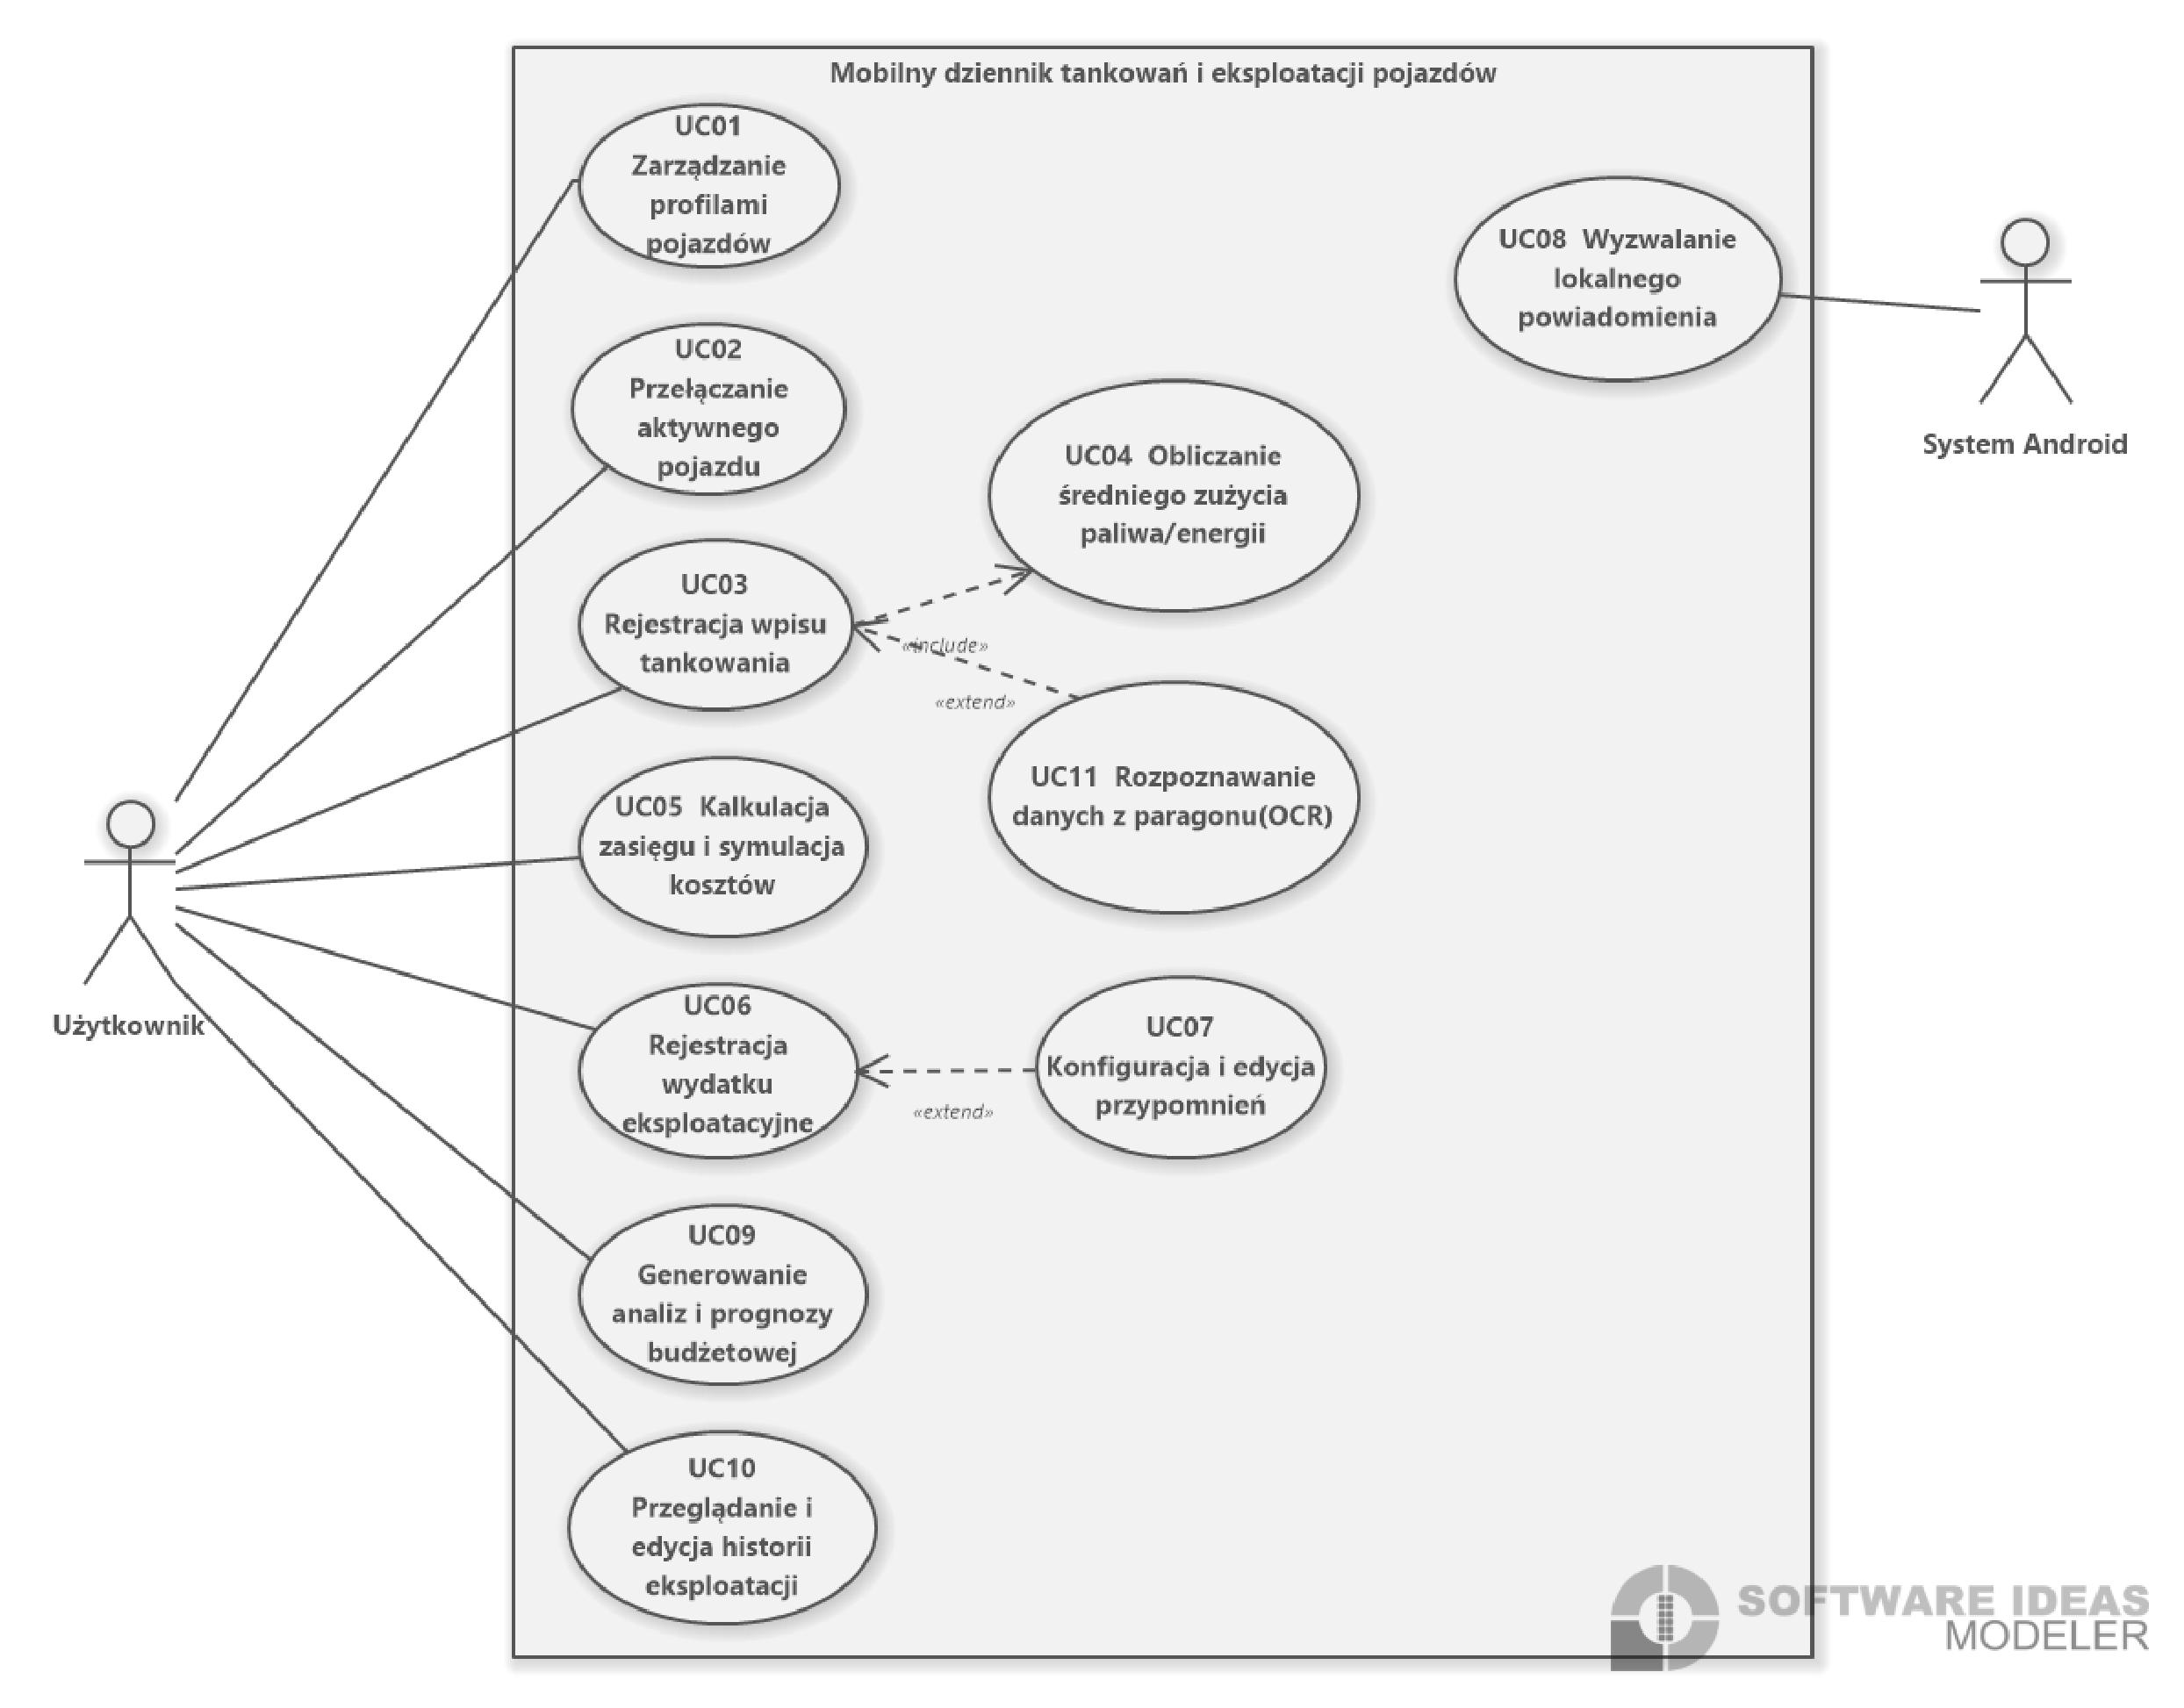
\includegraphics[width=0.98\linewidth]{figures/UseCaseDiagram1.eps}
    \caption{Diagram przypadków użycia}
    \label{fig:diagram_przypadkow_uzycia}
    \zrodlo{Opracowanie własne przy użyciu Software Ideas Modeler.}
\end{figure}

Na diagramie zastosowano relację «include» między przypadkami UC03 i~UC04 -- wyliczenie średniego zużycia paliwa/energii jest obowiązkowym elementem zapisu pełnego tankowania. Relację «extend» wykorzystano przy przypadkach UC11 (opcjonalne pobranie danych z~paragonu przez moduł OCR) oraz UC07 (opcjonalne zdefiniowanie przypomnienia podczas rejestracji wydatku). Pozostałe linie na diagramie stanowią asocjacje wskazujące udział aktorów w~realizacji poszczególnych operacji.

\clearpage

\subsection{Powiązanie wymagań funkcjonalnych z diagramem}
\label{subsec:powiazanie_wf_diagram}

Każde wymaganie funkcjonalne zdefiniowane w~rozdziale~\ref{cha:analiza_wymagan} znajduje odzwierciedlenie w~modelu przypadków użycia. Zestawienie powiązań przedstawiono w~tabeli~\ref{tab:powiazanie_wf_diagram}.

\begin{table}[H]
    \centering
    \caption{Powiązanie wymagań funkcjonalnych z~diagramem przypadków użycia}
    \label{tab:powiazanie_wf_diagram}
    \renewcommand{\arraystretch}{1.3}
    \begin{tabularx}{\linewidth}{|>{\centering\arraybackslash}p{1.5cm}|X|>{\centering\arraybackslash}p{2.6cm}|>{\centering\arraybackslash}p{2.2cm}|}
        \hline
        \rowcolor{tableheader}
        \textbf{ID} & \multicolumn{1}{c|}{\textbf{Wymaganie funkcjonalne}} & \textbf{Aktor} & \textbf{Przypadek użycia} \\
        \hline
        \hyperlink{wf:WF-01}{WF-01} & Dodawanie i~edycja profili pojazdów ze zdjęciem. & Użytkownik & \hyperlink{uc:UC01}{UC01} \\
        \hline
        \hyperlink{wf:WF-02}{WF-02} & Rejestracja tankowania z~automatycznym przeliczaniem kwot. & Użytkownik & \hyperlink{uc:UC03}{UC03} \\
        \hline
        \hyperlink{wf:WF-03}{WF-03} & Automatyczne obliczanie średniego zużycia paliwa/energii. & ------ & \hyperlink{uc:UC04}{UC04} \\
        \hline
        \hyperlink{wf:WF-04}{WF-04} & Wyliczanie przewidywanego zasięgu pojazdu. & Użytkownik & \hyperlink{uc:UC05}{UC05} \\
        \hline
        \hyperlink{wf:WF-05}{WF-05} & Rejestracja wydatków eksploatacyjnych z~kategoriami. & Użytkownik & \hyperlink{uc:UC06}{UC06} \\
        \hline
        \hyperlink{wf:WF-06}{WF-06} & Planowanie przypomnień i~wyzwalanie powiadomień w~tle. & Użytkownik / System Android & \hyperlink{uc:UC07}{UC07}, \hyperlink{uc:UC08}{UC08} \\
        \hline
        \hyperlink{wf:WF-07}{WF-07} & Generowanie miesięcznej prognozy wydatków. & Użytkownik & \hyperlink{uc:UC09}{UC09} \\
        \hline
        \hyperlink{wf:WF-08}{WF-08} & Przełączanie aktywnego widoku między pojazdami. & Użytkownik & \hyperlink{uc:UC02}{UC02} \\
        \hline
        \hyperlink{wf:WF-09}{WF-09} & Przeglądanie i~edycja historii eksploatacji. & Użytkownik & \hyperlink{uc:UC10}{UC10} \\
        \hline
        \hyperlink{wf:WF-10}{WF-10} & Zapis i~odczyt danych w~lokalnej bazie offline. & ------ & \hyperlink{uc:UC01}{UC01}, \hyperlink{uc:UC03}{UC03}, \hyperlink{uc:UC06}{UC06}, \hyperlink{uc:UC10}{UC10} \\
        \hline
        \hyperlink{wf:WF-11}{WF-11} & Skanowanie paragonu i~odczyt danych przez moduł OCR. & Użytkownik & \hyperlink{uc:UC11}{UC11} \\
        \hline
    \end{tabularx}
    \zrodlo{Opracowanie własne na podstawie analizy wymagań.}
\end{table}


\clearpage

\subsection{Szczegółowe specyfikacje przypadków użycia}
\label{subsec:scenariusze_przypadkow_uzycia}

W~niniejszej sekcji przedstawiono szczegółowe specyfikacje tabelaryczne dla dwóch wybranych przypadków użycia: przypadku UC03 (wykorzystującego relację «include») oraz przypadku UC06 (wykorzystującego relację «extend»).


\subsubsection{Specyfikacja przypadku użycia UC03: Rejestracja wpisu tankowania}
\label{subsubsec:specyfikacja_uc1}

Podstawowe parametry przypadku użycia UC03 zestawiono w~tabeli~\ref{tab:specyfikacja_uc1_parametry}.

\begin{table}[H]
    \centering
    \caption{Parametry przypadku użycia UC03}
    \label{tab:specyfikacja_uc1_parametry}
    \renewcommand{\arraystretch}{1.3}
    \begin{tabularx}{\linewidth}{|>{\bfseries\arraybackslash}p{4.2cm}|X|}
        \hline
        \rowcolor{tableheader}
        \multicolumn{1}{|c|}{\textbf{Element}} & \multicolumn{1}{c|}{\textbf{Opis}} \\
        \hline
        Identyfikator & UC03 \\
        \hline
        Nazwa & Rejestracja wpisu tankowania \\
        \hline
        Aktor główny & Użytkownik \\
        \hline
        Cel & Wprowadzenie danych o~zrealizowanym tankowaniu, aktualizacja stanu licznika pojazdu oraz obliczenie średniego zużycia paliwa/energii. \\
        \hline
        Warunki początkowe & Aplikacja jest uruchomiona, a~w~systemie istnieje co najmniej jeden aktywny profil pojazdu. \\
        \hline
        Powiązania & «include» UC04~--~Obliczenie średniego zużycia paliwa/energii, «extend» UC11~--~Rozpoznawanie danych z~paragonu (OCR) \\
        \hline
        Warunki końcowe -- sukces & Nowy wpis tankowania został zapisany w~bazie danych, stan licznika pojazdu zaktualizowany, a~w~przypadku tankowania do pełna wyliczono średnie spalanie. \\
        \hline
        Warunki końcowe -- niepowodzenie & Wpis nie został zapisany. System wyświetlił komunikat o~błędzie walidacji i~pozostawił formularz do poprawy. \\
        \hline
    \end{tabularx}
    \zrodlo{Opracowanie własne.}
\end{table}

\clearpage

Przebieg główny przypadku użycia przedstawiono w~tabeli~\ref{tab:przebieg_glowny_uc1}.

\begin{table}[H]
    \centering
    \caption{Przebieg główny przypadku użycia UC03}
    \label{tab:przebieg_glowny_uc1}
    \renewcommand{\arraystretch}{1.3}
    \begin{tabularx}{\linewidth}{|>{\centering\arraybackslash}p{1.2cm}|X|X|}
        \hline
        \rowcolor{tableheader}
        \textbf{Krok} & \multicolumn{1}{c|}{\textbf{Działanie aktora}} & \multicolumn{1}{c|}{\textbf{Odpowiedź systemu}} \\
        \hline
        1 & Wybiera opcję dodania nowego tankowania. & Wyświetla formularz z~podpowiedzią bieżącej daty i~ostatniego stanu licznika. \\
        \hline
        2 & Wprowadza stan licznika, ilość paliwa oraz łączny koszt (ręcznie lub skanując paragon przez \hyperlink{uc:UC11}{UC11}). & Na bieżąco przelicza cenę za litr przy zmianie kwoty (\hyperlink{rb:RB-04}{RB-04}). \\
        \hline
        3 & Zatwierdza formularz przyciskiem zapisu. & Sprawdza poprawność przebiegu (\hyperlink{rb:RB-01}{RB-01}) oraz daty (\hyperlink{rb:RB-05}{RB-05}) i~wylicza średnie spalanie (\hyperlink{uc:UC04}{UC04}, \hyperlink{rb:RB-02}{RB-02}). \\
        \hline
        4 & --- & Zapisuje wpis w~bazie danych (\hyperlink{wf:WF-10}{WF-10}) i~aktualizuje stan licznika pojazdu. \\
        \hline
        5 & --- & Wyświetla potwierdzenie zapisu, prezentuje wyliczone spalanie i~odświeża ekran główny. \\
        \hline
    \end{tabularx}
    \zrodlo{Opracowanie własne.}
\end{table}

\clearpage

Warianty alternatywne oraz obsługę wyjątków przedstawiono w~tabeli~\ref{tab:scenariusz_alt_uc1}.

\begin{table}[H]
    \centering
    \caption{Scenariusze alternatywne i~wyjątkowe dla przypadku użycia UC03}
    \label{tab:scenariusz_alt_uc1}
    \renewcommand{\arraystretch}{1.3}
    \begin{tabularx}{\linewidth}{|>{\centering\arraybackslash}p{1.4cm}|X|X|}
        \hline
        \rowcolor{tableheader}
        \textbf{Krok} & \multicolumn{1}{c|}{\textbf{Działanie aktora}} & \multicolumn{1}{c|}{\textbf{Odpowiedź systemu}} \\
        \hline
        \multicolumn{3}{|l|}{\cellcolor{tableheader!50}\textbf{Wariant A1 -- Stan licznika mniejszy od poprzedniego (\hyperlink{rb:RB-01}{RB-01})}} \\
        \hline
        A1.1 & --- & Wykrywa, że wprowadzony stan licznika jest mniejszy lub równy wartości z~poprzedniego wpisu. \\
        \hline
        A1.2 & --- & Blokuje zapis, podświetla pole przebiegu i~wyświetla komunikat błędu. \\
        \hline
        A1.3 & Poprawia wartość przebiegu. & Weryfikuje nową wartość i~usuwa komunikat błędu. \\
        \hline
        A1.4 & Ponownie zatwierdza formularz. & Powraca do weryfikacji w~kroku~3 przebiegu głównego. \\
        \hline
        \multicolumn{3}{|l|}{\cellcolor{tableheader!50}\textbf{Wariant A2 -- Rejestracja z~datą wsteczną (\hyperlink{rb:RB-05}{RB-05})}} \\
        \hline
        A2.1 & --- & Wykrywa, że data wpisu jest wcześniejsza niż data poprzedniego tankowania. \\
        \hline
        A2.2 & --- & Wyświetla okno ostrzegawcze o~możliwym zaburzeniu statystyk z~opcją kontynuacji lub anulowania. \\
        \hline
        A2.3 & Wybiera anulowanie zapisu lub potwierdza kontynuację. & Po anulowaniu umożliwia poprawę daty; po potwierdzeniu przechodzi do zapisu w~kroku~4. \\
        \hline
        A2.4 & Wprowadza skorygowaną datę i~ponawia zapis. & Powraca do kroku~3 przebiegu głównego. \\
        \hline
        \multicolumn{3}{|l|}{\cellcolor{tableheader!50}\textbf{Wariant A3 -- Niepełny odczyt danych z~paragonu (\hyperlink{uc:UC11}{UC11})}} \\
        \hline
        A3.1 & --- & Moduł OCR nie jest w~stanie poprawnie odczytać wszystkich pól z~fotografii. \\
        \hline
        A3.2 & --- & Wyświetla informację o~częściowym odczycie i~uzupełnia tylko rozpoznane wartości. \\
        \hline
        A3.3 & Ręcznie uzupełnia brakujące dane w~formularzu. & Sprawdza poprawność wprowadzonych wartości. \\
        \hline
        A3.4 & Zatwierdza uzupełniony formularz przyciskiem zapisu. & Powraca do kroku~3 przebiegu głównego. \\
        \hline
    \end{tabularx}
    \zrodlo{Opracowanie własne.}
\end{table}


\clearpage

\subsubsection{Specyfikacja przypadku użycia UC06: Rejestracja wydatku eksploatacyjnego}
\label{subsubsec:specyfikacja_uc2}

Podstawowe parametry przypadku użycia UC06 zestawiono w~tabeli~\ref{tab:specyfikacja_uc2_parametry}.

\begin{table}[H]
    \centering
    \caption{Parametry przypadku użycia UC06}
    \label{tab:specyfikacja_uc2_parametry}
    \renewcommand{\arraystretch}{1.3}
    \begin{tabularx}{\linewidth}{|>{\bfseries\arraybackslash}p{4.2cm}|X|}
        \hline
        \rowcolor{tableheader}
        \multicolumn{1}{|c|}{\textbf{Element}} & \multicolumn{1}{c|}{\textbf{Opis}} \\
        \hline
        Identyfikator & UC06 \\
        \hline
        Nazwa & Rejestracja wydatku eksploatacyjnego \\
        \hline
        Aktor główny & Użytkownik \\
        \hline
        Cel & Ewidencja kosztu eksploatacyjnego (np. naprawa, ubezpieczenie, badanie techniczne) z~możliwością zaplanowania przypomnienia o~nadchodzącym terminie. \\
        \hline
        Warunki początkowe & Aplikacja jest uruchomiona, a~w~systemie istnieje co najmniej jeden aktywny profil pojazdu. \\
        \hline
        Powiązania & «extend» UC07~--~Konfiguracja i~edycja przypomnień \\
        \hline
        Warunki końcowe -- sukces & Informacja o~wydatku została zapisana w~bazie danych, a~zaplanowane powiadomienia zarejestrowano w~systemie. \\
        \hline
        Warunki końcowe -- niepowodzenie & Wydatek nie został zapisany. System wyświetlił komunikat o~brakujących lub błędnych danych formularza. \\
        \hline
    \end{tabularx}
    \zrodlo{Opracowanie własne.}
\end{table}

Przebieg główny przypadku użycia przedstawiono w~tabeli~\ref{tab:przebieg_glowny_uc2}.

\begin{table}[H]
    \centering
    \caption{Przebieg główny przypadku użycia UC06}
    \label{tab:przebieg_glowny_uc2}
    \renewcommand{\arraystretch}{1.3}
    \begin{tabularx}{\linewidth}{|>{\centering\arraybackslash}p{1.2cm}|X|X|}
        \hline
        \rowcolor{tableheader}
        \textbf{Krok} & \multicolumn{1}{c|}{\textbf{Działanie aktora}} & \multicolumn{1}{c|}{\textbf{Odpowiedź systemu}} \\
        \hline
        1 & Przechodzi do modułu kosztów i~wybiera dodanie nowego wydatku. & Wyświetla formularz z~wyborem kategorii, kwotą, datą oraz opcją przypomnień. \\
        \hline
        2 & Wybiera kategorię okresową (np. ubezpieczenie), podaje kwotę i~datę. & Weryfikuje dane i~proponuje automatyczne przypomnienie 7~dni przed terminem (\hyperlink{rb:RB-03}{RB-03}). \\
        \hline
        3 & Przechodzi do konfiguracji przypomnień (\hyperlink{uc:UC07}{UC07}). & Umożliwia modyfikację terminu powiadomienia oraz dodanie kolejnych terminów. \\
        \hline
        4 & Zatwierdza formularz przyciskiem zapisu. & Zapisuje wydatek w~bazie danych (\hyperlink{wf:WF-10}{WF-10}) oraz rejestruje zaplanowane powiadomienia. \\
        \hline
        5 & --- & Wyświetla potwierdzenie zapisu i~odświeża listę wydatków. \\
        \hline
    \end{tabularx}
    \zrodlo{Opracowanie własne.}
\end{table}

\clearpage

Scenariusz alternatywny A1 dla przypadku UC06 przedstawiono w~tabeli~\ref{tab:scenariusz_alt_uc2}.

\begin{table}[H]
    \centering
    \caption{Scenariusz alternatywny A1 dla przypadku użycia UC06}
    \label{tab:scenariusz_alt_uc2}
    \renewcommand{\arraystretch}{1.3}
    \begin{tabularx}{\linewidth}{|>{\centering\arraybackslash}p{1.4cm}|X|X|}
        \hline
        \rowcolor{tableheader}
        \textbf{Krok} & \multicolumn{1}{c|}{\textbf{Działanie aktora}} & \multicolumn{1}{c|}{\textbf{Odpowiedź systemu}} \\
        \hline
        A1.1 & Pozostawia opcję przypomnień wyłączoną (np. wydatek jednorazowy). & Pomija konfigurację powiadomienia (\hyperlink{uc:UC07}{UC07}) i~oczekuje na zatwierdzenie. \\
        \hline
        A1.2 & Zatwierdza formularz przyciskiem zapisu. & Zapisuje wydatek w~bazie danych (\hyperlink{wf:WF-10}{WF-10}) bez planowania powiadomień. \\
        \hline
        A1.3 & --- & Wyświetla potwierdzenie zapisu i~odświeża listę wydatków. \\
        \hline
    \end{tabularx}
    \zrodlo{Opracowanie własne.}
\end{table}


\clearpage

% ==============================================================================
\section{Diagramy aktywności}
\label{sec:diagramy_aktywnosci}



% Diagramy aktywności (\emph{Activity Diagrams}) przedstawiają przepływ sterowania, logikę biznesową oraz sekwencję czynności wykonywanych w~ramach modelowanych procesów z~uwzględnieniem węzłów decyzyjnych oraz rozgałęzień współbieżnych.


% \subsection{Diagram aktywności 1: [Nazwa pierwszego procesu, np. Proces rejestracji tankowania i obliczania spalania]}
% \label{subsec:diagram_aktywnosci_1}

% % TODO: Wprowadzenie do modelowanego procesu, opis jego znaczenia w systemie.

% \begin{figure}[H]
%     \centering
%     % Miejsce na diagram aktywności 1
%     % \includegraphics[width=0.8\linewidth]{figures/fig_act_tankowanie.pdf}
%     \caption{Diagram aktywności procesu [Nazwa procesu 1]}
%     \label{fig:diagram_aktywnosci_1}
%     \zrodlo{Opracowanie własne.}
% \end{figure}




% TODO: Szczegółowy opis diagramu aktywności 1:
% - kolejność wykonywanych czynności od stanu początkowego,
% - warunki decyzyjne (np. walidacja poprawności przebiegu, sprawdzenie flagi "do pełna"),
% - alternatywne ścieżki i obsługa wyjątków,
% - osiągnięcie stanu końcowego.




% \subsection{Diagram aktywności 2: [Nazwa drugiego procesu, np. Proces harmonogramowania i wyzwalania powiadomień serwisowych]}
% \label{subsec:diagram_aktywnosci_2}

% % TODO: Wprowadzenie do drugiego modelowanego procesu.

% \begin{figure}[H]
%     \centering
%     % Miejsce na diagram aktywności 2
%     % \includegraphics[width=0.8\linewidth]{figures/fig_act_powiadomienia.pdf}
%     \caption{Diagram aktywności procesu [Nazwa procesu 2]}
%     \label{fig:diagram_aktywnosci_2}
%     \zrodlo{Opracowanie własne.}
% \end{figure}

% TODO: Szczegółowy opis diagramu aktywności 2:
% - sekwencja operacji (tworzenie wpisu z datą przypomnienia, rejestracja zadania w WorkManager),
% - warunki weryfikacji terminu (np. reguła 7 dni przed terminem - RB-03),
% - ścieżki alternatywne (edycja terminu, anulowanie zadania, oznaczenie opłaty jako załatwiona),
% - wygenerowanie powiadomienia w systemie Android i stan końcowy.

% \clearpage

% ==============================================================================
\section{Diagramy sekwencji}
\label{sec:diagramy_sekwencji}

% Diagramy sekwencji (\emph{Sequence Diagrams}) obrazują dynamiczne zachowanie systemu oraz czasowy przebieg interakcji i~komunikacji pomiędzy uczestnikami (aktorami, widokami interfejsu, modelami widoku oraz warstwą bazy danych).


% \subsection{Diagram sekwencji 1: [Nazwa pierwszej interakcji, np. Dodanie tankowania i aktualizacja statystyk pojazdu]}
% \label{subsec:diagram_sekwencji_1}

% % TODO: Wprowadzenie do modelowanej sekwencji interakcji.

% \begin{figure}[H]
%     \centering
%     % Miejsce na diagram sekwencji 1
%     % \includegraphics[width=0.9\linewidth]{figures/fig_seq_tankowanie.pdf}
%     \caption{Diagram sekwencji interakcji [Nazwa interakcji 1]}
%     \label{fig:diagram_sekwencji_1}
%     \zrodlo{Opracowanie własne.}
% \end{figure}

% % TODO: Opis przebiegu analizowanego scenariusza:
% % - identyfikacja uczestników (np. :Użytkownik, :AddRefuelingScreen, :RefuelingViewModel, :RefuelingRepository, :RoomDatabase),
% % - zestawienie i kolejność przesyłanych komunikatów synchronicznych i asynchronicznych,
% % - zwracane odpowiedzi, walidacja i odświeżenie stanu interfejsu (StateFlow).


% \subsection{Diagram sekwencji 2: [Nazwa drugiej interakcji, np. Rejestracja wydatku eksploatacyjnego i harmonogramowanie powiadomienia]}
% \label{subsec:diagram_sekwencji_2}

% % TODO: Wprowadzenie do drugiej modelowanej interakcji.

% \begin{figure}[H]
%     \centering
%     % Miejsce na diagram sekwencji 2
%     % \includegraphics[width=0.9\linewidth]{figures/fig_seq_powiadomienia.pdf}
%     \caption{Diagram sekwencji interakcji [Nazwa interakcji 2]}
%     \label{fig:diagram_sekwencji_2}
%     \zrodlo{Opracowanie własne.}
% \end{figure}

% % TODO: Opis przebiegu analizowanego scenariusza:
% % - uczestnicy (np. :Użytkownik, :ExpenseScreen, :ExpenseViewModel, :ExpenseRepository, :WorkManager),
% % - sekwencja wywołań metod i planowania powiadomienia w tle,
% % - komunikaty zwrotne i obsługa błędów.


% \clearpage

% ==============================================================================
\section{Diagramy stanów}
\label{sec:diagramy_stanow}

% Diagramy maszyny stanów (\emph{State Machine Diagrams}) modelują cykl życia wybranych obiektów systemu, których zachowanie zmienia się w~odpowiedzi na zachodzące zdarzenia i~operacje.


% \subsection{Diagram stanów 1: [Nazwa pierwszego obiektu, np. Cykl życia profilu pojazdu]}
% \label{subsec:diagram_stanow_1}

% % TODO: Opis obiektu, dla którego modelowany jest stan (uzasadnienie biznesowe).

% \begin{figure}[H]
%     \centering
%     % Miejsce na diagram stanów 1
%     % \includegraphics[width=0.8\linewidth]{figures/fig_state_pojazd.pdf}
%     \caption{Diagram stanów obiektu [Nazwa obiektu 1]}
%     \label{fig:diagram_stanow_1}
%     \zrodlo{Opracowanie własne.}
% \end{figure}

% % TODO: Opis stanów, zdarzeń i przejść:
% % - możliwe stany (np. NowyNieaktywowany, AktywnyDomyślny, WycofanyZEksploatacji / Archiwalny),
% % - zdarzenia wyzwalające przejścia (np. wybór jako aktywny profil, edycja danych, archiwizacja),
% % - warunki dozorujące (strażnicy / guards) i akcje wejściowe/wyjściowe.


% \subsection{Diagram stanów 2: [Nazwa drugiego obiektu, np. Cykl życia zobowiązania eksploatacyjnego / przypomnienia]}
% \label{subsec:diagram_stanow_2}

% % TODO: Opis drugiego obiektu (np. Zobowiązanie / Przypomnienie o przeglądzie lub polisie OC).

% \begin{figure}[H]
%     \centering
%     % Miejsce na diagram stanów 2
%     % \includegraphics[width=0.8\linewidth]{figures/fig_state_przypomnienie.pdf}
%     \caption{Diagram stanów obiektu [Nazwa obiektu 2]}
%     \label{fig:diagram_stanow_2}
%     \zrodlo{Opracowanie własne.}
% \end{figure}

% % TODO: Opis stanów, zdarzeń i przejść:
% % - stany obiektu (np. Zaplanowane, Oczekujące, WymagająceUwagi / Powiadomione, Zrealizowane / Opłacone, Przeterminowane),
% % - zdarzenia (np. upływ czasu, nadejście bufora 7 dni - RB-03, potwierdzenie opłaty przez kierowcę, edycja terminu),
% % - podsumowanie cyklu życia obiektu.

%\include{chapters/chapter004}


%------------------------------------------------------------------------------
% Bibliografia (przed spisami)
%------------------------------------------------------------------------------

\cleardoublepage
\begingroup
  \addcontentsline{toc}{chapter}{Bibliografia}
  \bibliographystyle{plainurl}
  \bibliography{bibliografia}
\endgroup

%------------------------------------------------------------------------------
% Spisy
%------------------------------------------------------------------------------

\cleardoublepage
\addcontentsline{toc}{chapter}{Spis rysunków}
\listoffigures

\cleardoublepage
\addcontentsline{toc}{chapter}{Spis tabel}
\listoftables

\cleardoublepage
\addcontentsline{toc}{chapter}{Spis listingów}
\lstlistoflistings




\end{document}